% Place in the appendix. The translation source sentence is original Chinese.
\begin{figure}[!t]
  \centering
  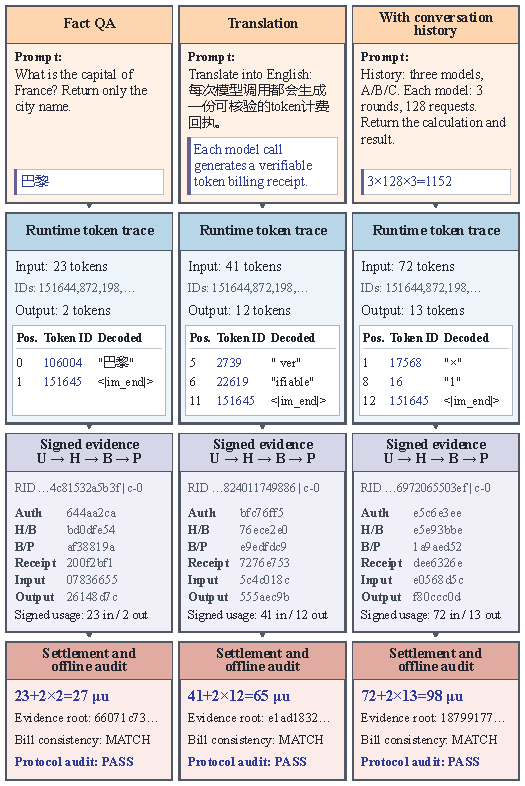
\includegraphics[width=\columnwidth]{token_provenance_case_boxes.pdf}
  \caption{Recorded token-billing provenance examples using Qwen3-14B.
  Each column follows a separate request through four layers: request/response,
  runtime token export, signed evidence, and settlement. The translation column
  reproduces the original Chinese source sentence; other prompts are English
  excerpts of the original messages. White insets show the responses verbatim.
  Token counts and IDs refer to the original recorded messages. Input counts
  include the chat template and, where applicable, conversation history; output
  counts include the end-of-message token. Output positions are zero-based and
  only the indicated positions are shown in the framed tables. Quotation marks
  delimit decoded text pieces, including leading spaces; \texttt{<|im\_end|>}
  is the end-of-message token.
  Auth, H/B, B/P, and Receipt identify the authorization, two bilateral handoffs,
  and provider receipt. RID suffixes and eight-hex-digit digest prefixes
  abbreviate full values available in the archived records. Experimental rates
  are one micro-unit per input token and two per output token. Receipts bind
  input/output digests and usage; token IDs are auxiliary runtime exports.
  The examples use host-generated role signatures and were collected separately
  from the performance measurements.}
  \label{fig:appendix-token-provenance-cases}
\end{figure}
